

\chapter{Release 2: Gestion des posts,des stories ,et des interactions sociales \& Le dashboard administrateur,un système de notifications.}
\label{chap_concep}

\minitoc

\DeclareRobustCommand{\greencheck}{%
  \tikz\fill[scale=0.4, color=green]
  (0,.35) -- (.25,0) -- (1,.7) -- (.25,.15) -- cycle;%
}

\section*{Introduction}
\addcontentsline{toc}{section}{Introduction}
Ce chapitre présente deux sprints clés du projet. Le premier concerne la gestion des posts, stories et interactions sociales (likes, commentaires), favorisant l’engagement entre utilisateurs. Le second porte sur la création d’un dashboard pour l’administrateur, offrant une vue globale sur les statistiques de la plateforme, ainsi que l’intégration d’un système de notifications pour informer les utilisateurs des activités importantes (commentaires, interactions, suggestions). Ces fonctionnalités renforcent la communication, la coordination et le suivi en temps réel sur la plateforme.




\section{Objectifs des Sprint 3 \& 4}



\subsection{Objectif du sprint 3 }

Le troisième sprint marque une étape clé dans l’amélioration de l’expérience utilisateur. Il a permis de créer un espace dédié à la gestion des posts et stories, avec l’intégration d’interactions sociales comme les likes et commentaires. L’objectif est de faire de la plateforme un véritable réseau interactif, favorisant l’expression et l’engagement.

Nous avons veillé à concevoir une interface moderne, ergonomique et réactive, encourageant les utilisateurs à créer et interagir facilement. Ce travail contribue à un environnement numérique vivant, au cœur de la stratégie de communication de l’application.



\subsection{Objectif du sprint 4}
Le quatrième sprint marque une étape stratégique avec l’implémentation d’un dashboard administrateur et d’un système de notifications. Le tableau de bord offre une vue globale en temps réel sur l’activité de la plateforme, incluant les utilisateurs actifs, les publications, les interactions et les statistiques clés, facilitant ainsi le pilotage et la prise de décision. En parallèle, le système de notifications informe l’utilisateur des actions le concernant (messages, commentaires, mises à jour), renforçant ainsi l’engagement et la réactivité. Ce sprint contribue à améliorer à la fois la supervision côté administrateur et la communication côté utilisateur.


\section{ Backlog Fonctionnel – Sprints 3 \& 4}
\subsection{Backlog Produit – Gestion des posts \&  des stories \& des interactions sociales }


\setlength{\LTpre}{0pt}
\setlength{\LTpost}{0pt}

\renewcommand{\arraystretch}{1.3}

\begin{longtable}{|p{4cm}|p{8cm}|p{2cm}|p{3cm}|}

\hline
\textbf{User Story} & \textbf{Description} & \textbf{Priorité} \\
\hline
\endfirsthead

\hline
\textbf{User Story} & \textbf{Description} & \textbf{Priorité} \\
\hline
\endhead

\hline
\endfoot

\hline
\endlastfoot

US-16 & En tant qu'utilisateur, je peux pouvoir publier du contenu textuel dans mon domaine professionnel. & Haute \\
\hline
US-17 & En tant qu'utilisateur, je peux pouvoir publier des images, vidéos  à mes publications. & Moyenne \\
\hline
US-18 & En tant qu'utilisateur, je peux pouvoir ajouter des hashtags à mes posts pour améliorer leur visibilité. & Basse \\
\hline
US-19 & En tant qu'utilisateur, je peux pouvoir ajouter des tags à mes posts pour améliorer leur visibilité. & Basse \\
\hline
US-20 & En tant qu'utilisateur, je peux pouvoir joindre un lien (URL) à mes posts pour partager des ressources ou rediriger vers du contenu externe. & Moyenne \\
\hline
US-21 & En tant qu'utilisateur, je peux pouvoir supprimer mes posts. & Haute \\
\hline
US-22 & En tant qu'utilisateur, je peux pouvoir consulter les posts des autres utilisateurs que je suis. & Moyenne \\
\hline
US-23 & En tant qu'utilisateur, je peux pouvoir rechercher des posts par mots-clés. & Moyenne \\
\hline
US-24 & En tant qu'utilisateur, je peux pouvoir aimer les publications d'autres utilisateurs. & Moyenne \\
\hline
US-25 & En tant qu'utilisateur, je peux pouvoir commenter les publications. & Moyenne \\
\hline
US-26 & En tant qu'utilisateur, je peux pouvoir supprimer mes propres commentaires pour corriger une erreur ou retirer une intervention. & Basse \\
\hline
US-27 & En tant qu'utilisateur, je peux pouvoir voir le nombre total de likes reçus sur tous les posts afin d'évaluer la popularité des publications. & Moyenne \\
\hline
US-28 & En tant qu'utilisateur, je peux pouvoir voir le nombre total de commentaires reçus sur tous les posts afin de mesurer le niveau d'interaction. & Moyenne \\
\hline
US-29 & En tant qu'utilisateur, je peux pouvoir répondre aux commentaires sur les posts. & Basse \\
\hline
US-30 & En tant qu'utilisateur, je peux pouvoir voir qui a aimé mes publications. & Basse \\
\hline
US-31 & En tant qu'utilisateur, je peux pouvoir partager les publications d'autres utilisateurs. & Basse \\
\hline
US-32 & En tant qu'utilisateur, je peux pouvoir créer des stories textuelles éphémères avec personnalisation de couleurs. & Moyenne \\
\hline
US-33 & En tant qu'utilisateur, je peux pouvoir créer des stories avec des images. & Moyenne \\
\hline
US-34 & En tant qu'utilisateur, je peux pouvoir créer des stories avec des vidéos. & Moyenne \\
\hline
US-35 & En tant qu'utilisateur, je peux voir combien de personnes ont vu mes stories et qui exactement. & Basse \\
\hline
US-36 & En tant qu'utilisateur, je peux être alerté lorsqu'un utilisateur que je suis a publié une nouvelle story. & Moyenne \\
\hline
US-37 & En tant qu'utilisateur, je peux pouvoir voir les stories des utilisateurs que je suis. & Moyenne \\
\hline
US-38 & En tant qu'utilisateur, je peux que mes stories expirent automatiquement après 24 heures. & Haute \\
\hline
US-39 & En tant qu'utilisateur, je peux pouvoir supprimer mes stories pour retirer un contenu que je ne souhaite plus partager. & Moyenne \\
\hline
US-40 & En tant qu'utilisateur, je peux pouvoir supprimer mes stories pour retirer un contenu que je ne souhaite plus partager. & Moyenne \\
\hline
US-41 & En tant qu'utilisateur, je peux voir un fil d'actualité avec les publications des utilisateurs que je suis. & Haute \\
\hline
US-42 & En tant qu'utilisateur, je peux pouvoir filtrer mon fil d'actualité par domaine professionnel. & Moyenne \\
\hline
US-43 & En tant qu'utilisateur, je peux voir les publications les plus populaires dans mon domaine. & Basse \\
\hline
US-44 & En tant qu'utilisateur, je peux un fil d'actualité qui se met à jour en temps réel. & Moyenne \\
\hline 
\caption{Liste des User Stories} \label{tab:userstories} \\
\end{longtable}
\subsection{Backlog Produit – Le dashboard administrateur \&  un système de notifications }
\begin{table}[H]
\centering
\begin{tabularx}{\textwidth}{|c|X|c|}
\hline
\textbf{User Story} & \textbf{Description} & \textbf{Priorité} \\
\hline
US-45 & En tant qu'administrateur, je peux avoir accès à un tableau de bord avec des statistiques sur l'activité des utilisateurs. & Moyenne \\
\hline
US-46 & En tant qu'administrateur, je peux voir des métriques sur les publications des utilisateurs (vues, likes, commentaires). & Moyenne \\
\hline
US-47 & En tant qu'administrateur, je peux voir des statistiques sur les offres d'emploi et projets publiés. & Moyenne \\
\hline
US-48 & En tant qu'administrateur, je peux consulter des graphiques sur l'engagement global avec les publications et offres. & Basse \\
\hline
US-49 & En tant qu'administrateur, je peux voir des statistiques globales sur la plateforme. & Basse \\
\hline

US-50 & En tant qu'utilisateur, je peux recevoir des notifications pour les nouvelles interactions sur mes publications. & Haute \\
\hline
US-51 & En tant qu'utilisateur, je peux recevoir des notifications pour les nouveaux abonnés. & Moyenne \\
\hline
US-52 & En tant qu'utilisateur, je peux pouvoir marquer des notifications individuelles comme lues. & Moyenne \\
\hline
US-53 & En tant qu'utilisateur, je peux pouvoir marquer toutes mes notifications comme lues en un clic. & Moyenne \\
\hline
US-54 & En tant qu'utilisateur, je peux pouvoir voir le nombre de notifications non lues. & Haute \\
\hline
US-55 & En tant qu'utilisateur, je peux pouvoir supprimer des notifications individuelles. & Basse \\
\hline
US-56 & En tant qu'utilisateur, je peux pouvoir supprimer toutes mes notifications en un clic. & Basse \\
\hline
US-57 & En tant qu'utilisateur, je peux recevoir des notifications en temps réel. & Haute \\
\hline
\end{tabularx}
\caption{User Stories liées au tableau de bord (administrateur) et aux notifications (utilisateur)}
\end{table}

\section{ Raffinement des cas d'utilisation }
\subsection{Raffinement des cas d'utilisation de sprint 1 }
\subsubsection{Raffinement de cas d'utilisation Gestion post}
la figure 4.1 présente le raffinement de cas d'utilisation Gestion post,suivie par leur description textuelle dans le tableau 4.2
\begin{figure}[H]
    \centering
    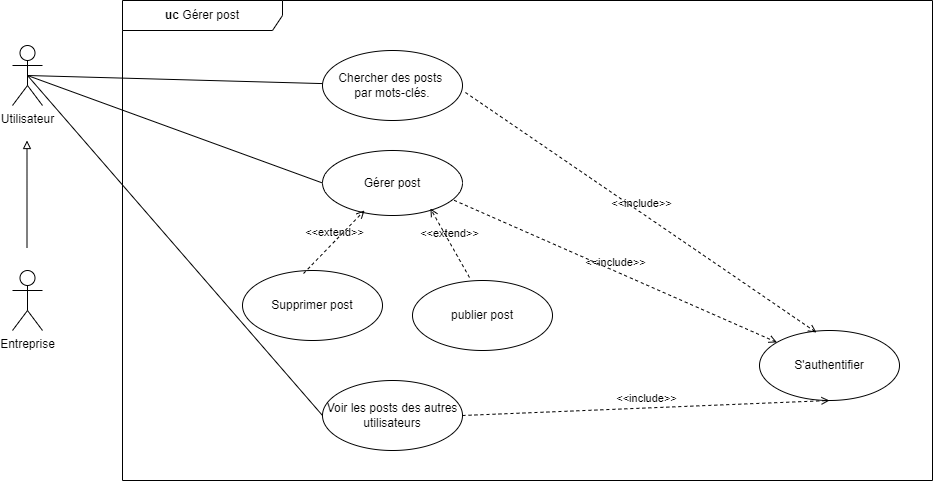
\includegraphics[width=1\textwidth]{images/Diagramme gerer postsfinale1.drawio.png}
    \caption{Diagramme de cas d'utilisation de Gestion post}
    \label{fig:chap4_post_refinement}
\end{figure}
Le cas d’utilisation "Publier un post" permet à l’utilisateur de partager du contenu sur la plateforme sous différentes formes : texte, image, ou vidéo. Lors de la création du post, l’utilisateur peut enrichir sa publication en ajoutant des hashtags, des émoticônes, ou encore en joignant une URL pour fournir des références ou rediriger vers d’autres contenus.

\begin{table}[h!]
\centering
\begin{tabular}{|p{4cm}|p{10cm}|}
\hline
\textbf{Élément}        & \textbf{Description} \\ \hline
Cas d'utilisation       & Publier post \\ \hline
Acteur                  & Utilisateur \\ \hline
Précondition            & L'utilisateur doit être authentifié pour pouvoir publier un post. \\ \hline
Postcondition           & Le post est enregistré dans le système et visible selon la configuration choisie (profil ou fil d'actualité). \\ \hline
Scénario nominal        & 
1. L'utilisateur clique sur « Publier ». \newline
2. Le système affiche l'interface de création de post. \newline
3. L'utilisateur saisit un texte, ajoute éventuellement une image ou une vidéo. \newline
4. L'utilisateur peut ajouter des hashtags, des emojis et/ou un lien. \newline
5. L'utilisateur choisit où publier le post (profil ou fil d'actualité). \newline
6. Le système enregistre le post et l'affiche dans la section choisie. \\ \hline

Scénario alternatif     & 
1a. Si l'utilisateur n'est pas connecté, le système le redirige vers la page d'authentification. \newline
2a. Si le post est vide, le système empêche la publication et demande à l'utilisateur d'ajouter du contenu. \\ \hline
\end{tabular}
\caption{Description textuelle du cas d'utilisation Publier post}
\end{table}

 
\subsubsection{Raffinement de cas d'utilisation Gestion Story}
la figure 4.2 présente le raffinement de cas d'utilisation Gestion story,suivie par leur description textuelle dans le tableau 4.3
\begin{figure}[H]
    \centering
    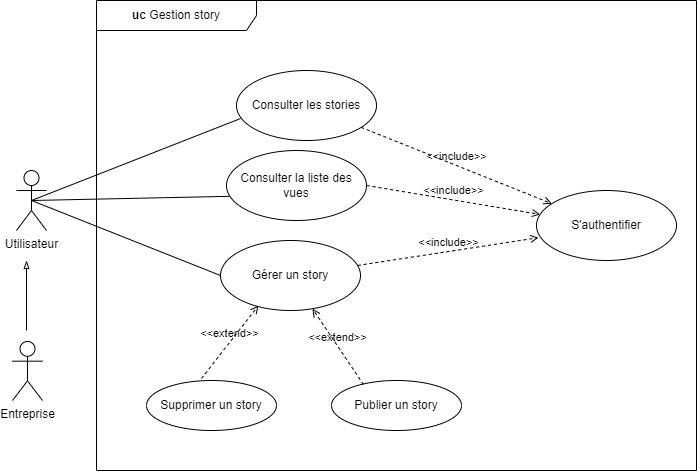
\includegraphics[width=1\textwidth]{images/Diagramme gerer storyfinale1.drawio.png}
    \caption{Diagramme de cas d'utilisation de Gestion story}
    \label{fig:chap4_story_refinement}
\end{figure}
Le cas d’utilisation "Gérer une story" permet à l’utilisateur de publier du contenu éphémère sous forme de texte, image ou courte vidéo. Les stories offrent un moyen rapide et expressif de partager des moments ou des idées, sans encombrer le fil principal. Elles sont temporaires et disparaissent automatiquement après 24 heures, renforçant l’aspect spontané et dynamique de l’interaction sur la plateforme. Cette fonctionnalité vise à stimuler l’engagement quotidien tout en offrant un espace de communication plus libre et instantané.


\begin{table}[h!]
\centering
\begin{tabular}{|p{4cm}|p{10cm}|}
\hline
\textbf{Élément} & \textbf{Description} \\ \hline
Cas d'utilisation & Publier une story \\ \hline
Acteur & Utilisateur \\ \hline
Postcondition & La story est publiée et visible par les utilisateurs abonnés pendant 24 heures. \\ \hline
Scénario nominal & 1. L'utilisateur ouvre l'interface story. \newline 2. Le système affiche l'interface de création de story. \newline 3. L'utilisateur choisit le type de contenu (texte/image/vidéo). \newline 4. L'utilisateur saisit/sélectionne le contenu et publie. \newline 5. Le système enregistre et rend la story disponible temporairement. \\ \hline
Scénario alternatif & 1a. Si l'utilisateur n'est pas connecté, le système redirige vers la page de connexion. \newline 3a. Si aucun contenu n'est ajouté, le système empêche la publication et demande à l'utilisateur d'ajouter un contenu. \\ \hline
\end{tabular}
\caption{Description textuelle du cas d'utilisation Publier une story}
\end{table}
\begin{figure}[H]
    \centering
    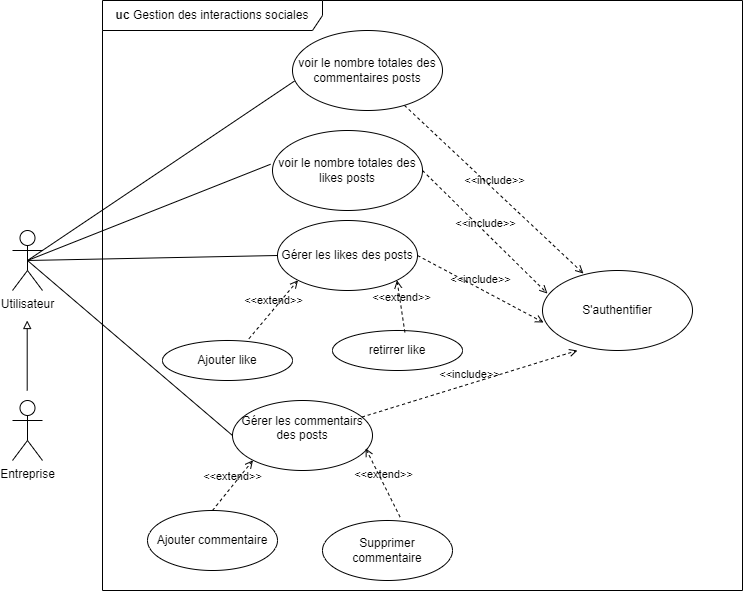
\includegraphics[width=1\textwidth]{images/Diagramme gestion des interactions socialesfinale1.drawio.png}
    \caption{Diagramme de cas d'utilisation de Gestion des interactions sociales}
    \label{fig:chap4_social_refinement}
\end{figure}

\begin{table}[h!]
\centering
\begin{tabular}{|p{4cm}|p{10cm}|}
\hline
\textbf{Élément} & \textbf{Description} \\ \hline
Cas d'utilisation & Ajouter like \\ \hline
Acteur & Utilisateur \\ \hline
Précondition & L'utilisateur doit être authentifié et accéder à un post. \\ \hline
Postcondition & Le like est ajouté ou retiré selon l'action. \\ \hline
Scénario nominal & 1. L'utilisateur clique sur le bouton de like. \newline 2. Le système vérifie si l'utilisateur a déjà liké. \newline 3a. Si ce n'est pas le cas, un like est ajouté. \newline 3b. Sinon, le like est retiré. \\ \hline
Scénario alternatif & 1a. Si l'utilisateur n'est pas authentifié, il est redirigé vers la page de connexion. \newline 2a. Si une erreur réseau survient, le like n'est pas enregistré. \\ \hline
\end{tabular}
\caption{Description du cas d'utilisation : Gérer les likes des posts}
\end{table}
\subsection{Raffinement des cas d'utilisation de sprint 2 }
\subsection{Raffinement de cas d'utilisation de Gestion de dashboard administrateur}
Voici le raffinement du diagramme de cas d'utilisation relatif à la gestion du dashboard administrateur, afin de mieux définir les interactions possibles et les fonctionnalités spécifiques réservées à ce rôle. 
\begin{figure}[H]
    \centering
    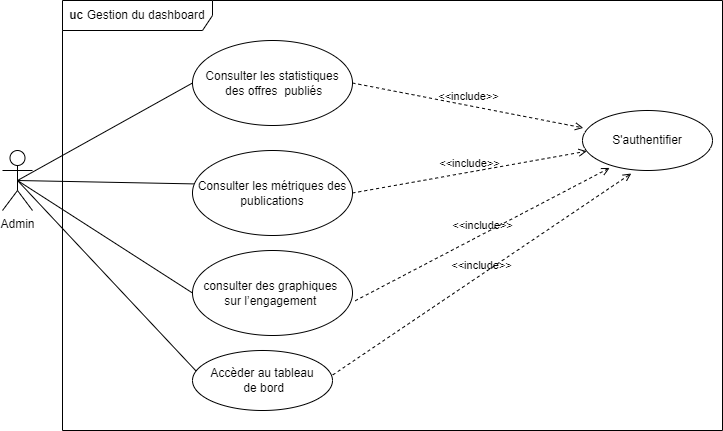
\includegraphics[width=1\textwidth]{images/Diagramme gestion dashboard.finaledrawio.png}
    \caption{Diagramme de cas d'utilisation de Gestion du dashboard}
    \label{fig:chap4_dashboard_refinement}
\end{figure}
\begin{table}[h!]
\centering
\begin{tabular}{|p{4cm}|p{10cm}|}
\hline
\textbf{Élément} & \textbf{Description} \\ \hline
Cas d'utilisation & Consulter les métriques sur des publications . \\ \hline
Acteur & Admin \\ \hline
Précondition & L'admin est authentifié et a accès au tableau de bord. \\ \hline
Postcondition & Les métriques relatives aux publications des utilisateurs sont affichées à l'admin sous forme de données chiffrées et/ou graphiques. \\ \hline
Scénario nominal & 
1. L'admin accède au tableau de bord. \newline
2. Il sélectionne l'option «Consulter les métriques des publications». \newline
3. Le système interroge la base de données. \newline
4. Les données sont traitées et formatées. \newline
5. Le système affiche les métriques sous forme de tableaux ou graphiques. \\ \hline
Scénario alternatif & 
1a. Si les données sont indisponibles (ex. erreur de serveur ou base vide), le système affiche un message d'erreur. \newline
2a. L'admin peut réessayer ultérieurement ou contacter le support technique. \\ \hline
\end{tabular}
\caption{Description textuelle du cas d'utilisation : Voir les métriques sur les publications des utilisateurs}
\end{table}
\subsection{Raffinement de cas d'utilisation de Gestion de Systéme de notification}
\begin{figure}[H]
    \centering
    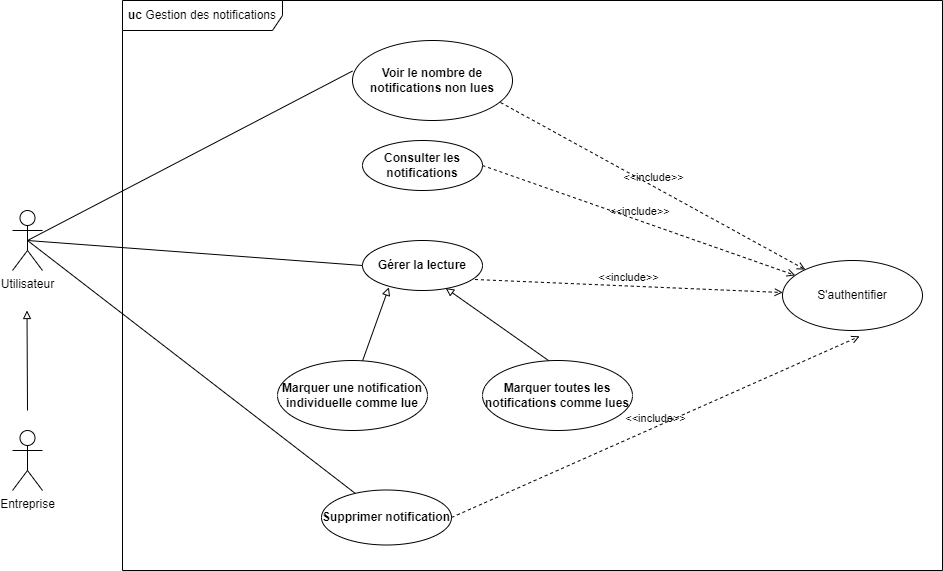
\includegraphics[width=1\textwidth]{images/Diagramme gestion notificationdrawiofinale1.drawio.png}
    \caption{Diagramme de cas d'utilisation de Gestion de Systéme de notification}
    \label{fig:chap4_notifications_refinement}
\end{figure}
Le tableau ci-dessous présente en détail le cas d'utilisation « Recevoir des notifications pour les nouveaux abonnés », décrivant ses préconditions, postconditions, scénario nominal et scénarios alternatifs.
\begin{table}[h!]
\centering
\begin{tabular}{|p{4cm}|p{10cm}|}
\hline
\textbf{Élément} & \textbf{Description} \\ \hline
Cas d'utilisation & Consulter les notifications \\ \hline
Acteur & Utilisateur \\ \hline
Précondition & L’utilisateur doit être authentifié sur la plateforme. \\ \hline
Postcondition & La liste des notifications est affichée à l’utilisateur. \\ \hline
Scénario nominal & 
1. L’utilisateur accède à la plateforme. \newline
2. Il clique sur l’icône ou le menu "Notifications". \newline
3. Le système vérifie l’authentification. \newline
4. Le système affiche les notifications disponibles (lues et non lues). \\ \hline
Scénario alternatif & 
1a. Si l’utilisateur n’est pas authentifié, il est redirigé vers la page de connexion. \\ \hline
\end{tabular}
\caption{Description du cas d'utilisation : Consulter les notifications}
\end{table}


\section{Détails des cas d'utilisation}
\subsection{Détails des cas d'utilisation du sprint 1}

\subsubsection{Cas d'utilisation : Gestion post}
La figure~\ref{fig:chap4_post_refinement} présente le diagramme du cas d'utilisation "Publier post".
\begin{figure}[H]
    \centering
    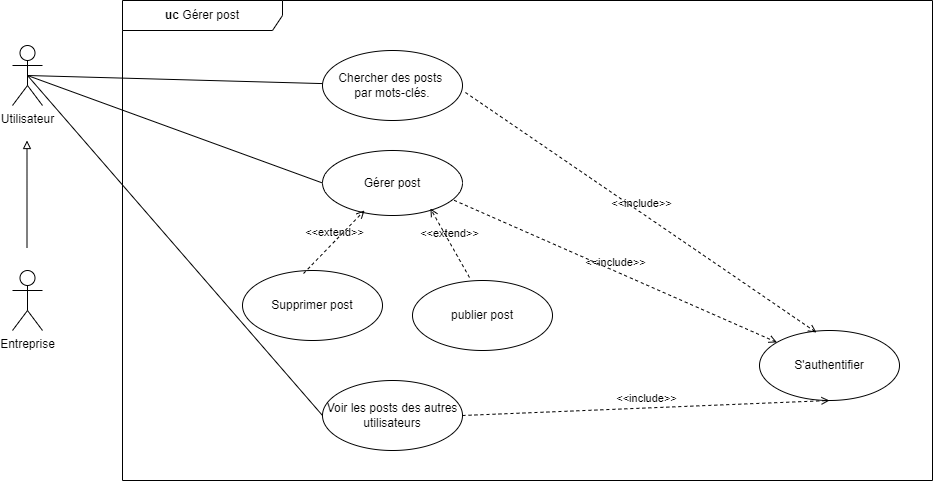
\includegraphics[width=1\textwidth]{images/Diagramme gerer postsfinale1.drawio.png}
    \caption{Diagramme de cas d'utilisation de Gestion post}
    \label{fig:chap4_post_refinement}
\end{figure}

\begin{table}[h!]
\centering
\begin{tabular}{|p{4cm}|p{10cm}|}
\hline
	extbf{Élément} & \textbf{Description} \\ \hline
Cas d'utilisation & Publier post \\ \hline
Acteur & Utilisateur \\ \hline
Précondition & L'utilisateur doit être authentifié pour pouvoir publier un post. \\ \hline
Postcondition & Le post est enregistré dans le système et visible selon la configuration choisie (profil ou fil d'actualité). \\ \hline
Scénario nominal & 1. L'utilisateur clique sur « Publier ». \\ 2. Le système affiche l'interface de création de post. \\ 3. L'utilisateur saisit le contenu et/ou ajoute une image/vidéo. \\ 4. L'utilisateur peut ajouter hashtags / emojis / lien. \\ 5. Le système enregistre et affiche le post. \\ \hline
Scénario alternatif & 1a. Si l'utilisateur n'est pas connecté, redirection vers l'authentification. \\ 2a. Si le post est vide, publication empêchée. \\ \hline
\end{tabular}
\caption{Description textuelle du cas d'utilisation Publier post}
\end{table}

\subsubsection{Cas d'utilisation : Gestion Story}
La figure~\ref{fig:chap4_story_refinement} présente le diagramme du cas d'utilisation "Gérer une story".
\begin{figure}[H]
    \centering
    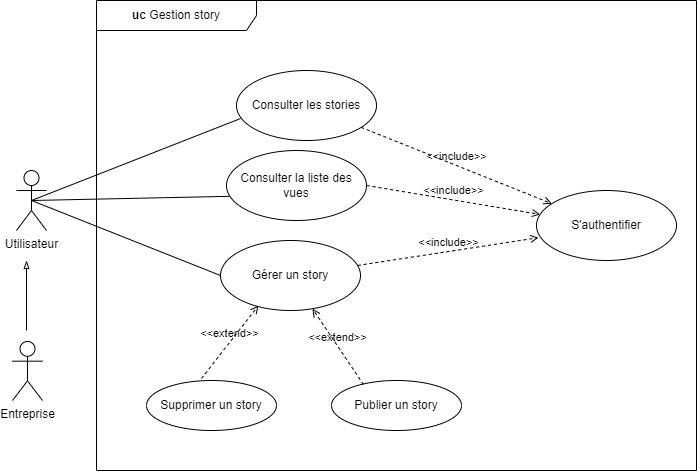
\includegraphics[width=1\textwidth]{images/Diagramme gerer storyfinale1.drawio.png}
    \caption{Diagramme de cas d'utilisation de Gestion story}
    \label{fig:chap4_story_refinement}
\end{figure}

\begin{table}[h!]
\centering
\begin{tabular}{|p{4cm}|p{10cm}|}
\hline
	extbf{Élément} & \textbf{Description} \\ \hline
Cas d'utilisation & Publier une story \\ \hline
Acteur & Utilisateur \\ \hline
Précondition & L'utilisateur est authentifié. \\ \hline
Postcondition & La story est publiée et visible pendant 24 heures par les abonnés. \\ \hline
Scénario nominal & 1. L'utilisateur ouvre l'interface story. \\ 2. Il choisit le type de contenu (texte/image/vidéo). \\ 3. Il saisit/sélectionne le contenu et publie. \\ 4. Le système enregistre et rend la story disponible temporairement. \\ \hline
Scénario alternatif & 1a. Si non authentifié, redirection. \\ 2a. Si aucun contenu, publication empêchée. \\ \hline
\end{tabular}
\caption{Description textuelle du cas d'utilisation : Publier une story}
\end{table}

\subsubsection{Cas d'utilisation : Gestion des interactions sociales}
La figure~\ref{fig:chap4_social_refinement} présente le diagramme des interactions sociales.
\begin{figure}[H]
    \centering
    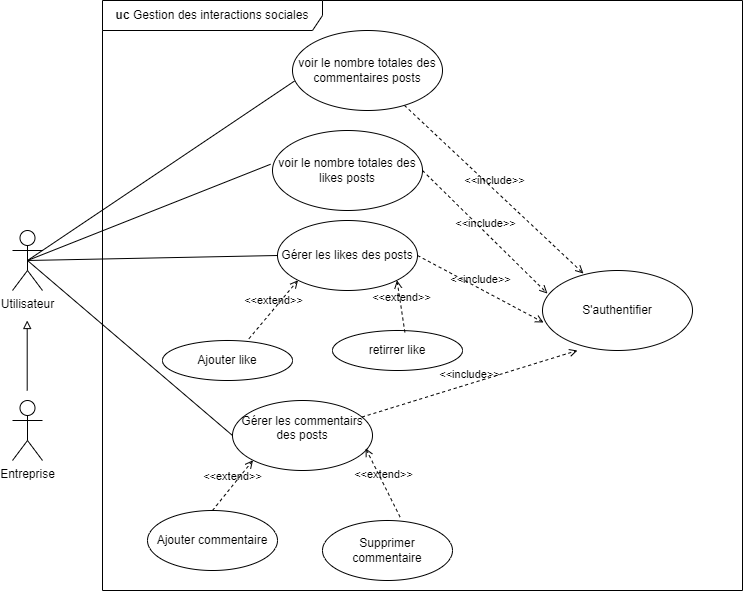
\includegraphics[width=1\textwidth]{images/Diagramme gestion des interactions socialesfinale1.drawio.png}
    \caption{Diagramme de cas d'utilisation de Gestion des interactions sociales}
    \label{fig:chap4_social_refinement}
\end{figure}

\begin{table}[h!]
\centering
\begin{tabular}{|p{4cm}|p{10cm}|}
\hline
	extbf{Élément} & \textbf{Description} \\ \hline
Cas d'utilisation & Ajouter/retirer un like \\ \hline
Acteur & Utilisateur \\ \hline
Précondition & L'utilisateur est authentifié et visualise un post. \\ \hline
Postcondition & Le like est ajouté ou retiré. \\ \hline
Scénario nominal & 1. L'utilisateur clique sur le bouton like. \\ 2. Le système met à jour l'état du like. \\ \hline
Scénario alternatif & 1a. Si non authentifié, redirection. \\ 2a. En cas d'erreur réseau, action non sauvegardée. \\ \hline
\end{tabular}
\caption{Description du cas d'utilisation : Gérer les likes des posts}
\end{table}

\subsection{Détails des cas d'utilisation du sprint 2}

\subsubsection{Cas d'utilisation : Gestion du dashboard administrateur}
\begin{figure}[H]
    \centering
    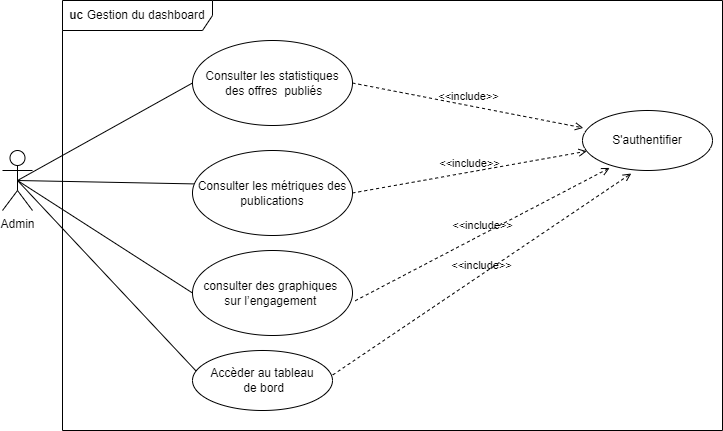
\includegraphics[width=1\textwidth]{images/Diagramme gestion dashboard.finaledrawio.png}
    \caption{Diagramme de cas d'utilisation de Gestion du dashboard}
    \label{fig:chap4_dashboard_refinement}
\end{figure}

\begin{table}[h!]
\centering
\begin{tabular}{|p{4cm}|p{10cm}|}
\hline
	extbf{Élément} & \textbf{Description} \\ \hline
Cas d'utilisation & Consulter les métriques sur des publications \\ \hline
Acteur & Administrateur \\ \hline
Précondition & L'admin est authentifié et a accès au tableau de bord. \\ \hline
Postcondition & Les métriques sont affichées sous forme de tableaux ou graphiques. \\ \hline
Scénario nominal & 1. L'admin accède au tableau de bord. \\ 2. Il sélectionne l'option de métriques. \\ 3. Le système affiche les données. \\ \hline
Scénario alternatif & 1a. Si données indisponibles, afficher message d'erreur. \\ \hline
\end{tabular}
\caption{Description textuelle du cas d'utilisation : Voir les métriques}
\end{table}

\subsubsection{Cas d'utilisation : Consulter les notifications}
\begin{figure}[H]
    \centering
    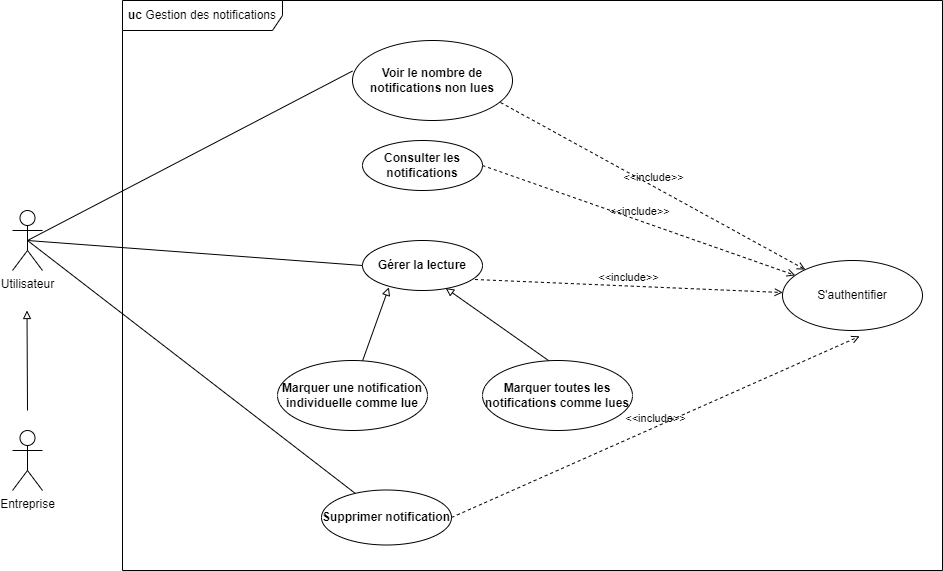
\includegraphics[width=1\textwidth]{images/Diagramme gestion notificationdrawiofinale1.drawio.png}
    \caption{Diagramme de cas d'utilisation de Gestion de Système de notification}
    \label{fig:chap4_notifications_refinement}
\end{figure}

\begin{table}[h!]
\centering
\begin{tabular}{|p{4cm}|p{10cm}|}
\hline
	extbf{Élément} & \textbf{Description} \\ \hline
Cas d'utilisation & Consulter les notifications \\ \hline
Acteur & Utilisateur \\ \hline
Précondition & L’utilisateur est authentifié. \\ \hline
Postcondition & La liste des notifications est affichée. \\ \hline
Scénario nominal & 1. L’utilisateur clique sur l’icône Notifications. \\ 2. Le système affiche les notifications (lues et non lues). \\ \hline
Scénario alternatif & 1a. Si non authentifié, redirection vers la page de connexion. \\ \hline
\end{tabular}
\caption{Description du cas d'utilisation : Consulter les notifications}
\end{table}



























